\chapter{Machine Learning Modeling Review}
\label{ch2}
PyTorch reference \cite{NEURIPS2019_9015}.
\section{Fundamentals of Training and Testing}
\begin{figure}[h!]
	\centering
		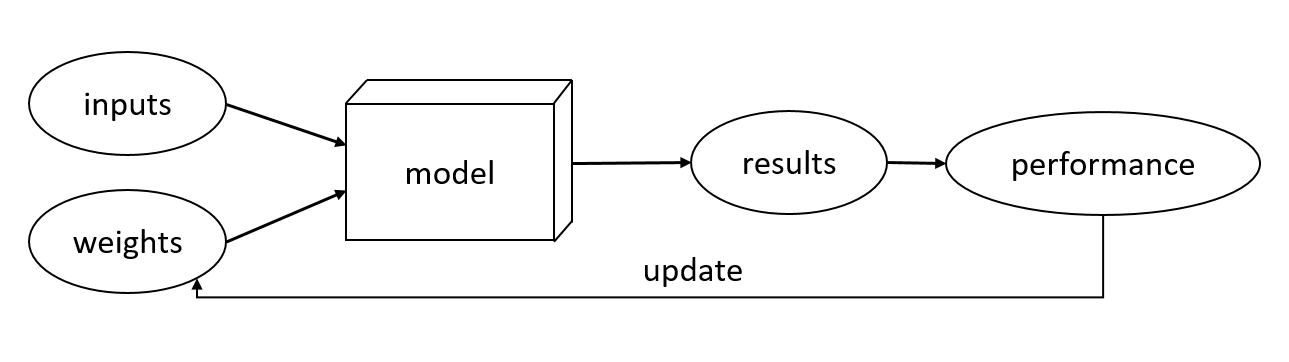
\includegraphics[width=0.99\textwidth]
		{training_process.png}
		\hfill
		\caption{Simple example of machine learning model training .}
		\label{fig:simple_model_training}
\end{figure}

\begin{figure}[h!]
	\centering
	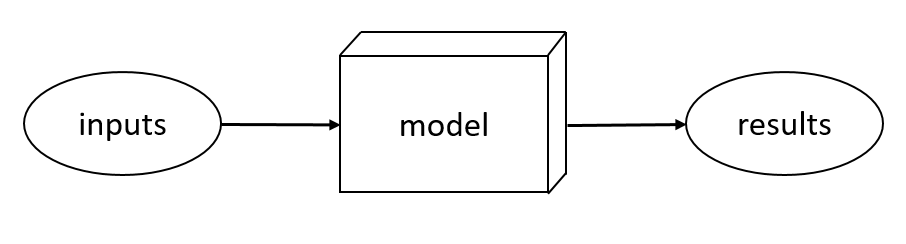
\includegraphics[width=0.99\textwidth]
	{testing_process.png}
	\hfill
	\caption{Simple example of machine learning model testing.}
	\label{fig:simple_model_testing}
\end{figure}

%\begin{figure}[h!]
%	\centering
%	\subfloat[Training\label{fig:simple_model_training_testing_a}]{
%		\includegraphics[width=0.99\textwidth]
%		{training_process.png}
%	}
%	\hfill
%	\subfloat[Testing\label{fig:simple_model_training_testing_b}]{
%		\includegraphics[width=0.99\textwidth]
%		{testing_process.png}
%	}
%	\hfill
%	\caption{Simple example of machine learning model training and testing.}
%	\label{fig:simple_model_training_testing}
%\end{figure}

\section{MLP and RNN Architectures}
\subsection{MLP}
\begin{equation} \label{eq:MLP}
	y = \sigma \left(xW + b\right)
\end{equation}
where $x$ is the input, $W$ is the learnable weights and $b$ is the learnable bias.

\subsection{RNN}
A recurrent neural network (RNN) is a neural network that operates on a variable-length sequence. The RNN processes the sequence input with a hidden state $h$ whose activation (value) at each time $t$ is dependent on the activation of the previous time. At each time step $t$ the hidden state $h_{t}$ of the RNN is updated by
\begin{equation} \label{eq:RNN}
	h_{t} = \tanh\left(W_{ih}x_{t} + b_{ih} + W_{hh}h_{\left(t-1\right)} + b_{hh}\right)
\end{equation}
where $x_{t}$ is the input at time $t$, $h_{\left(t-1\right)}$ is the hidden state of the previous layer at time $t-1$ or the initial state at time 0 (zero), $W_{ih}$ is the learnable input-hidden weights, $b_{ih}$ is the learnable input-hidden bias, $W_{hh}$ is the learnable hidden-hidden weights, and $b_{hh}$ is the learnable hidden-hidden bias \cite{NEURIPS2019_9015}.

\subsection{LSTM}
For each element in the input sequence, each layer computes the following function:
\begin{align}
	i_{t} &= \sigma\left(W_{ii}x_{t} + b_{ii} + W_{hi}h_{\left(t-1\right)} + b_{hi}\right) \label{eq:LSTM1} \\
	f_{t} &= \sigma\left(W_{if}x_{t} + b_{if} + W_{hf}h_{\left(t-1\right)} + b_{hf}\right) \label{eq:LSTM2} \\
	g_{t} &= \tanh\left(W_{ig}x_{t} + b_{ig} + W_{hg}h_{\left(t-1\right)} + b_{hg}\right) \label{eq:LSTM3} \\
	o_{t} &= \sigma\left(W_{io}x_{t} + b_{io} + W_{ho}h_{\left(t-1\right)} + b_{ho}\right) \label{eq:LSTM4} \\
	c_{t} &= f_{t} \odot c_{\left(t-1\right)} + i_{t} \odot g_{t} \label{eq:LSTM5} \\
	h_{t} &= o_{t} \odot \tanh\left(c_{t}\right) \label{eq:LSTM6}
\end{align}
where $h_{t}$ is the hidden state at time $t$, $c_{t}$ is the cell state at time $t$, $x_{t}$ is the input at time $t$, $h_{\left(t-1\right)}$ is the hidden state of the layer at time $t-1$ or the initial state at time 0 (zero), and $i_{t}$, $f_{t}$, $g_{t}$, and $o_{t}$ are the input, forget, cell, and output gates, respectively. $W_{ii}$, $W_{if}$, $W_{ig}$, and $W_{io}$ are the learnable input-hidden weights for the input, forget, cell, and output gates. $\sigma$ is the sigmoid function, and $\odot$ is the Hadamard (element-wise) product \cite{NEURIPS2019_9015}.

\subsection{GRU}
For each element in the input sequence, each layer computes the following function:
\begin{align}
	r_{t} &= \sigma\left(W_{ir}x_{t} + b_{ir} + W_{hr}h_{\left(t-1\right)} + b_{hr}\right) \label{eq:GRU1} \\
	z_{t} &= \sigma\left(W_{iz}x_{t} + b_{iz} + W_{hz}h_{\left(t-1\right)} + b_{hz}\right) \label{eq:GRU2} \\
	n_{t} &= \tanh\left(W_{in}x_{t} + b_{in} + r_{t} \odot \left(W_{hn}h_{\left(t-1\right)} b_{hn}\right)\right) \label{eq:GRU3} \\
	h_{t} &= \left(1 - z_{t}\right) \odot n_{t} + z_{t} \odot h_{\left(t-1\right)} \label{eq:GRU4}
\end{align}
where $h_{t}$ is the hidden state at time $t$, $x_{t}$ is the input at time $t$, $h_{\left(t-1\right)}$ is the hidden state of the layer at time $t-1$ or the initial hidden state at time 0 (zero), and $r_{t}$, $z_{t}$, and $n_{t}$ are the reset, update, and new gates, respectively. $W_{ir}$, $W_{iz}$ and $W_{in}$ are the learnable input-hidden weights for the reset, update, and new gates, respectively, and are of shape $numlayers \times 3hiddensize \times inputsize$. $W_{hr}$, $W_{hz}$ and $W_{hn}$ are the learnable hidden-hidden weights for the reset, update, and new gates, respectively, and are of shape $numlayers \times 3hiddensize \times inputsize$. $b_{ir}$, $b_{iz}$, and $b_{in}$ are the learnable input-hidden biases of the reset, update, and new gates, respectively. $b_{hr}$, $b_{hz}$, and $b_{hn}$ are the learnable hidden-hidden biases of the reset, update, and new gates, respectively. $\sigma$ is the sigmoid function, and $\odot$ is the Hadamard (element-wise) product \cite{NEURIPS2019_9015}. 

\section{Optimization and Loss Function}
Neural networks are a collection of nested functions that are executed on some input data. These functions are defined by \emph{parameters} (weights and biases). The training of a neural network is the process of updating the parameters to reduce the loss between network outputs and truth values. Training happens in two steps. The first step is forward propagation in which the network makes a prediction by passing input values through its functions (applying the weights and biases). The second step is backward propagation where the network adjusts its parameters proportionate to the error in its prediction. The network does this by moving backwards through the network from the output, collecting the derivatives of the error with respect to the parameters of the functions and optimizing the parameters using gradient descent. The derivatives of the error with respect to the parameters are called gradients. PyTorch's automatic differentiation engine \textit{autograd} handles this entire process \cite{NEURIPS2019_9015}.

Follow 3Blue1Brown video but with my own images and notations. Start with a 1x1 then move to a 2x2 network?
``These chain rule expressions give you the derivatives that determine each component in the gradient that helps minimize the loss of the network by repeatedly stepping downhill." - 3Blue1Brown

\section{Chapter Summary?}